\documentclass[
]{beamer}

\usepackage[english, russian]{babel}
\usepackage[utf8]{inputenc}
\usepackage[T1]{fontenc}
\usepackage{csquotes}
\usepackage{expl3,biblatex}
\usepackage{booktabs}
\usepackage{graphicx}
\usepackage{hyperref}

\title{Методы исследования черных дыр}

\author[]{Егор Горяной}
\begin{document}

\begin{frame}[plain]
\maketitle
\end{frame}
\begin{frame}{Черная дыра}
Черная дыра - астрономический объект с настолько сильной гравитацией, что ничего, включая кванты света, не может покинуть её. Граница этой области называется горизонтом событий.
\begin{figure}[H]
	\centering
	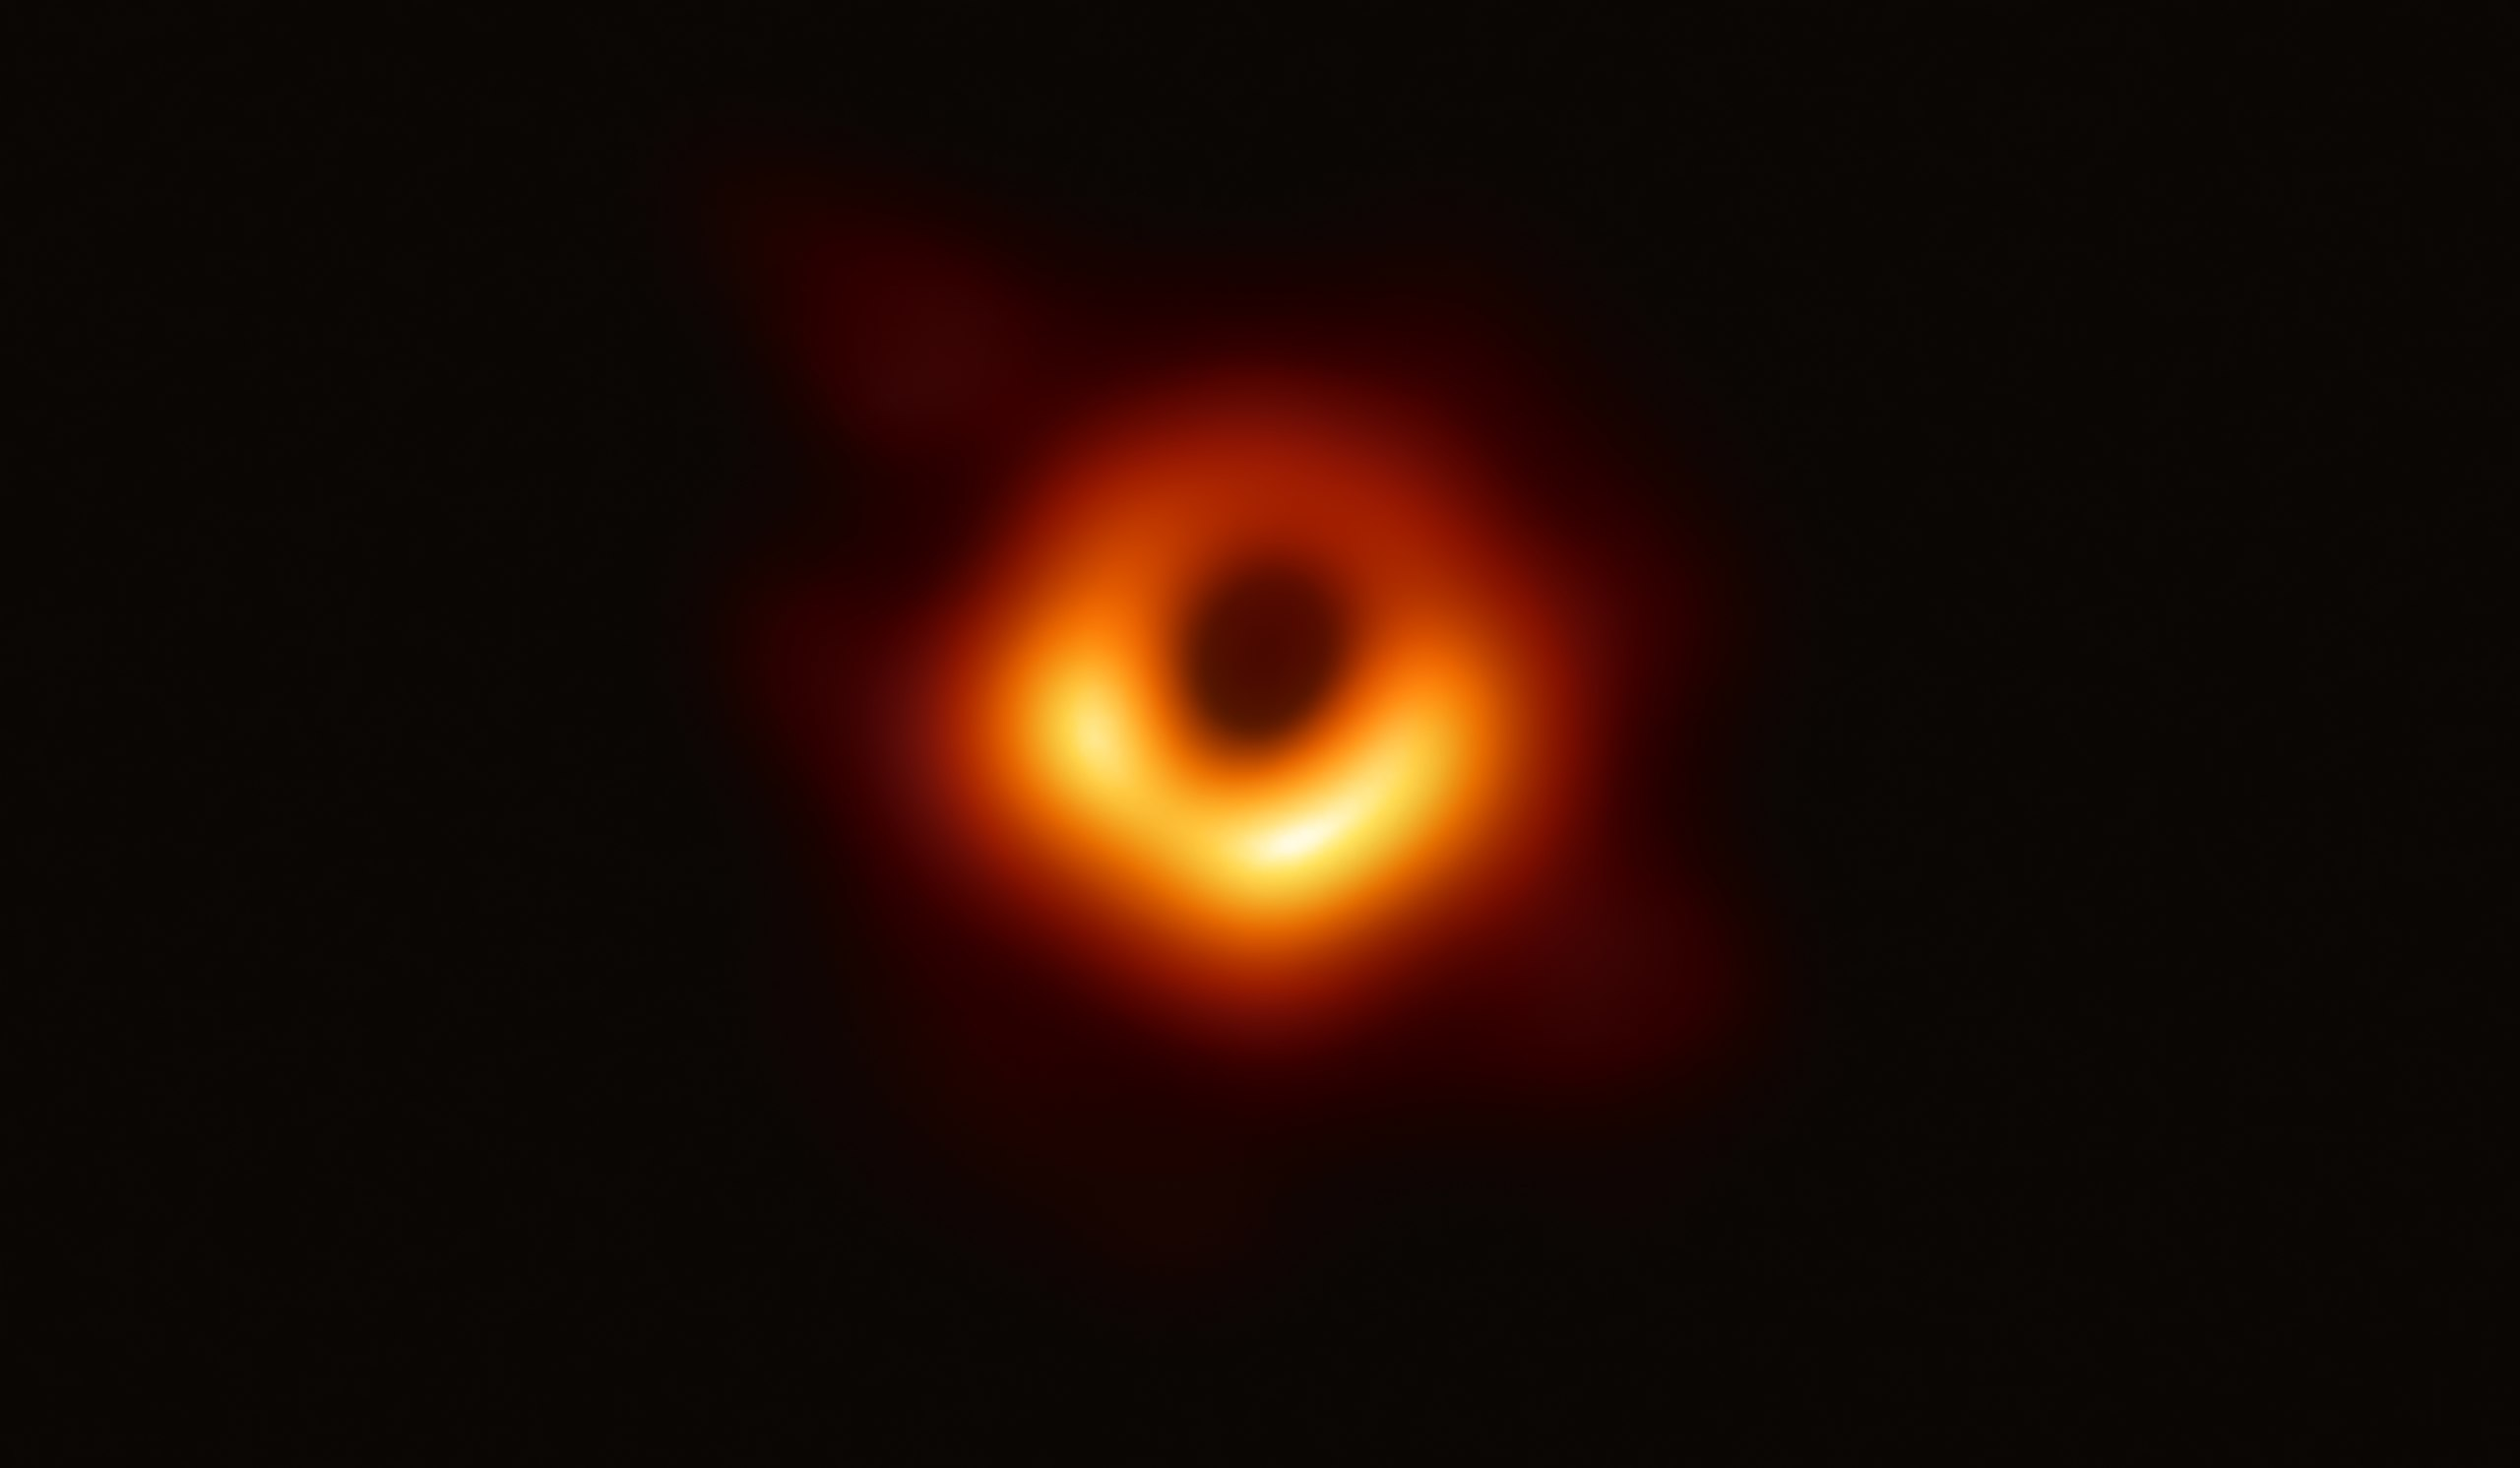
\includegraphics[width=7cm, height=5cm]{Black_hole_-_Messier_87.jpg}
	\caption{Сверхмассивная черная дыра в центре галактики М87}
\end{figure}
\end{frame}


\begin{frame}{Уравнения Эйнштейна}
\[R_{\mu\nu}-\frac{R}{2}g_{\mu\nu}+\Lambda g_{\mu\nu}=\frac{8\pi G}{c^4}T_{\mu\nu}\]
\begin{itemize}
    \item $R_{\mu\nu}$ - тензор кривизны Риччи
    \item $R$ - скалярная кривизна($R=g^{\mu\nu}R_{\mu\nu}$)
    \item $g_{\mu\nu}$ - метрический тензор
    \item $T_{\mu\nu}$ - тензор энергии-импульса
    \item $\Lambda$ - космологическая постоянная
\end{itemize}
\end{frame}

\begin{frame}{Решение Шварцшильда}
$T_{\mu\nu}=0,~\Lambda=0,~r_s=\displaystyle\frac{2GM}{c^2}$
\newline
\newline
\newline
$g=$
$\begin{pmatrix}
(1-\frac{r_s}{r}) & 0 & 0 & 0\\
0 & -(1-\frac{r_s}{r})^{-1} & 0 & 0\\
0 & 0 & -r^2 & 0\\
0 & 0 & 0 & -r^2\sin^2\theta\\
\end{pmatrix}$
\newline
\newline
\newline
$ds^2=(1-\frac{r_s}{r})c^2dt^2-\displaystyle\frac{dr^2}{(1-\frac{r_s}{r})}
-r^2(d\theta^2+\sin^2\theta d\varphi^2)$
\newline
\newline
\newline
\href{https://www.youtube.com/watch?v=3NFqXgH-4tg}{Более подробные математические выкладки}
\end{frame}

\begin{frame}{Гравитационное линзирование}
$L_0=[\sqrt{r(r-r_s)}+r_s\ln{(\sqrt{r}+\sqrt{r-r_s})}]^{r_2}_{r_1}$
\begin{figure}[H]
	\centering
	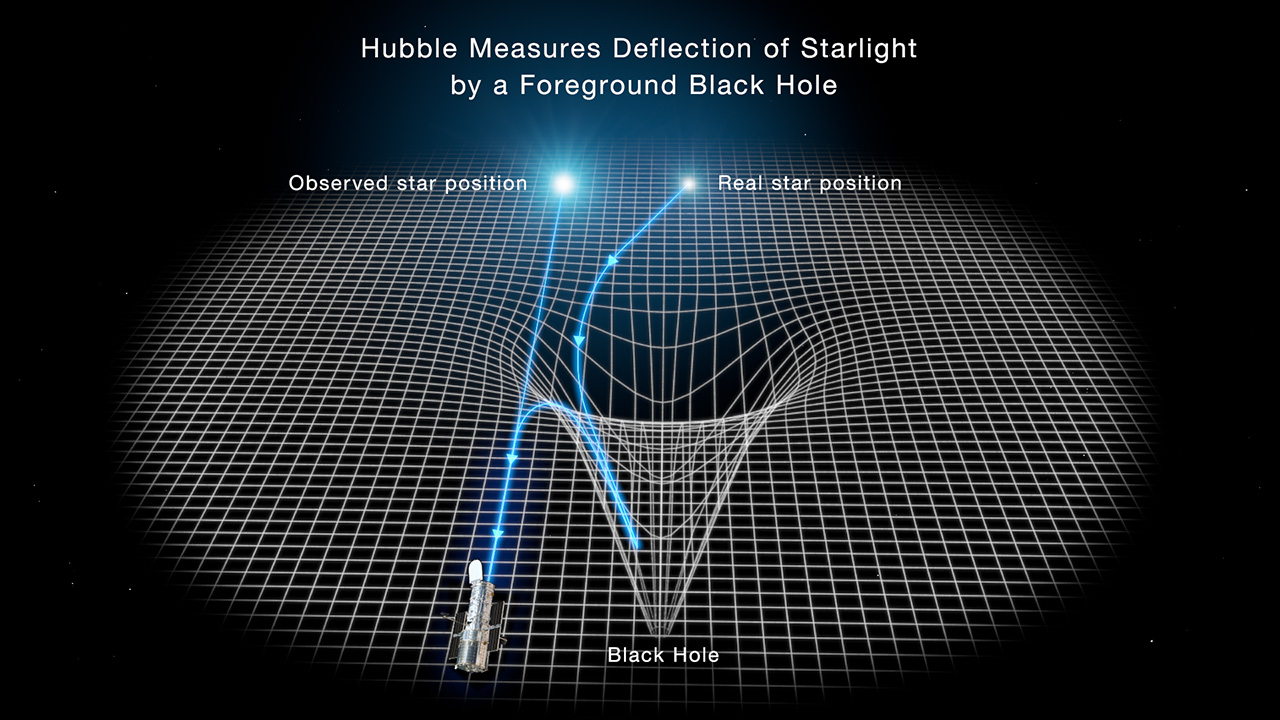
\includegraphics[width=5cm, height=5cm]{Gravitational_lensing_by_a_black_hole.jpg}
	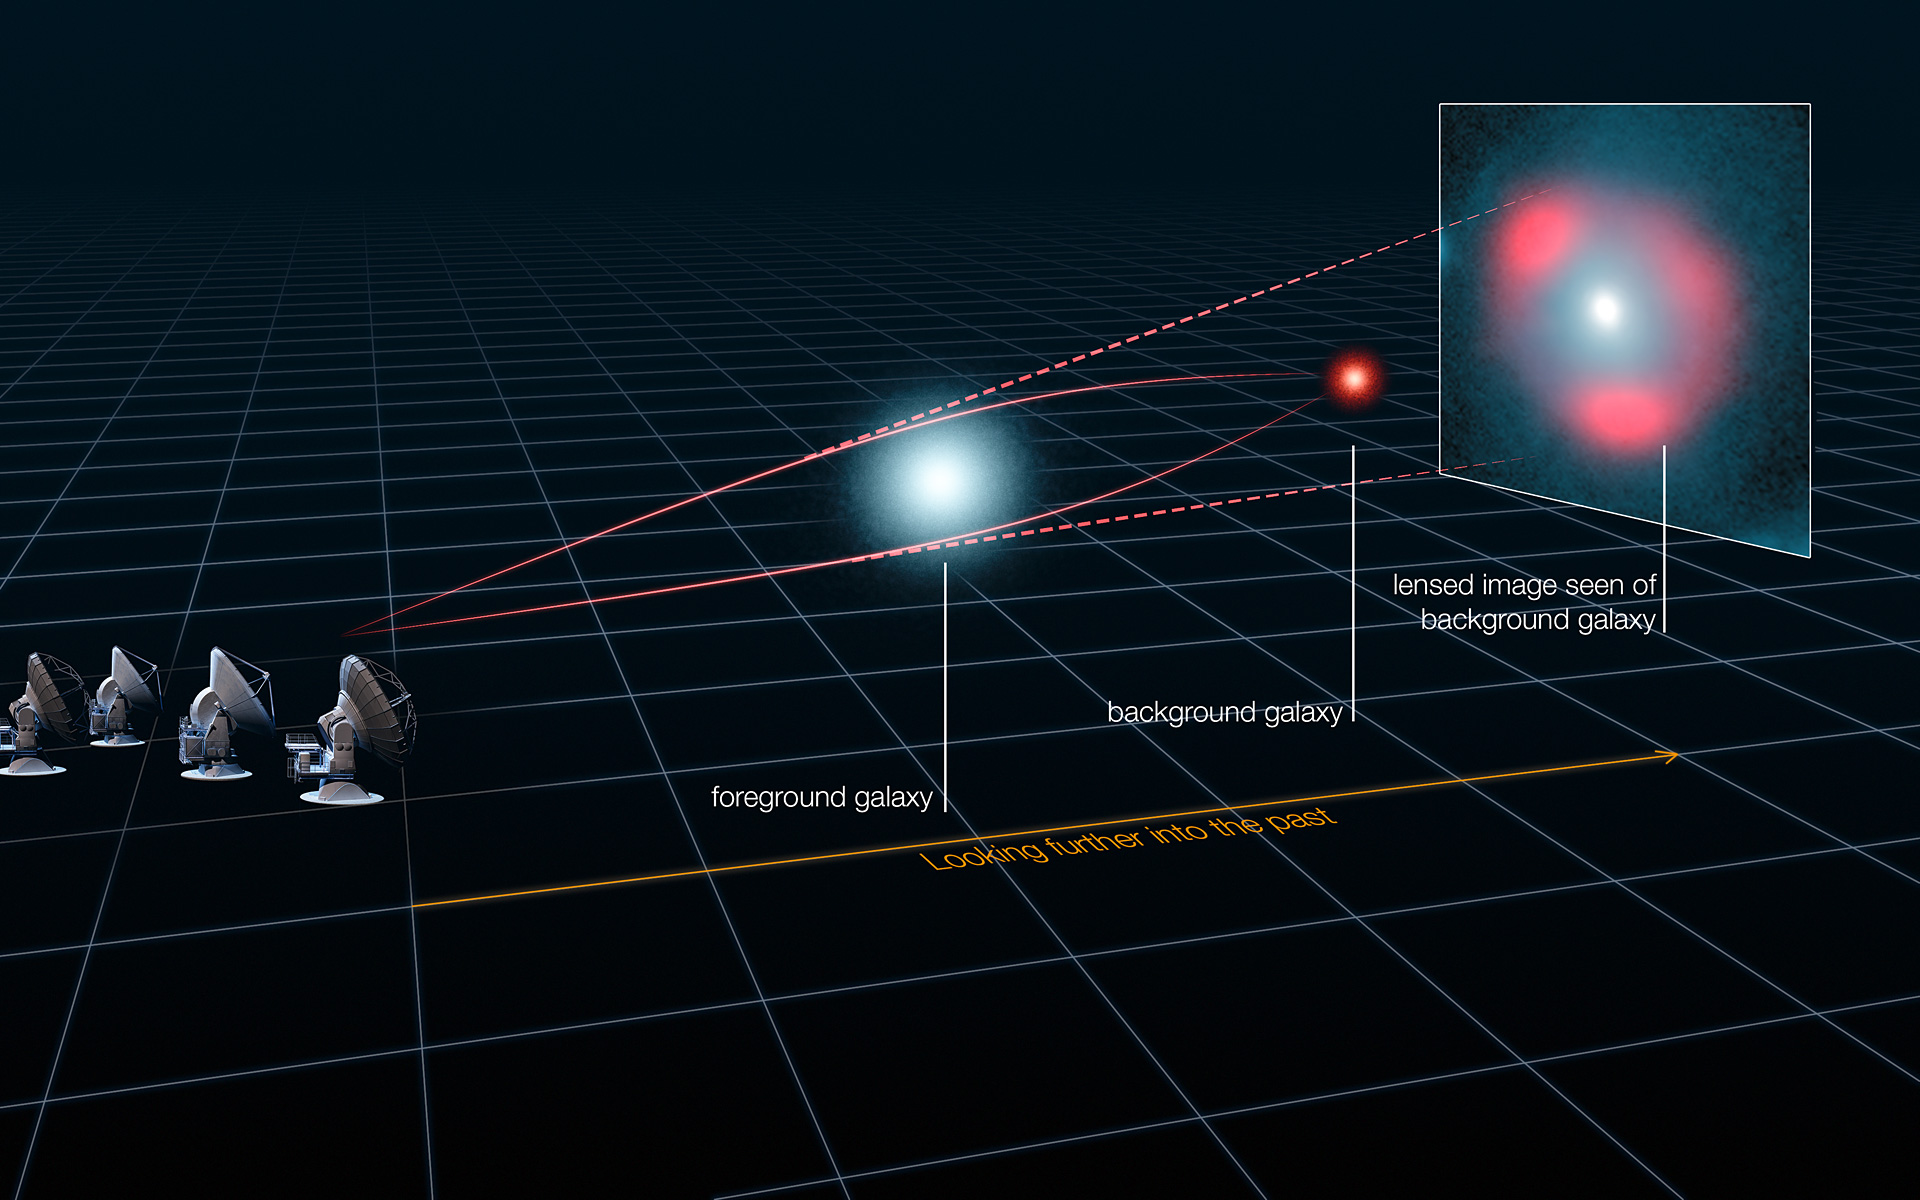
\includegraphics[width=5cm, height=5cm]{NCTjtDGTTWDt3m2pDBoa2Z.jpg}
	\caption{Геометрия гравитационной линзы}
\end{figure}
\end{frame}
\begin{frame}
\begin{figure}[H]
	\centering
	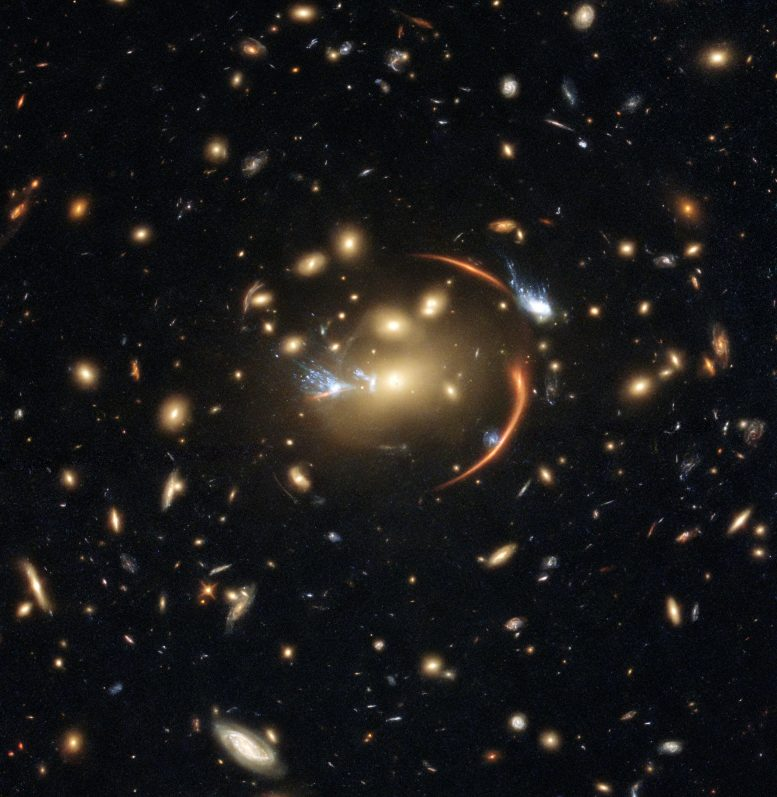
\includegraphics[width=5cm, height=5cm]{Galaxy-Cluster-MACSJ0138-0-2155-777x797-1.jpg}
	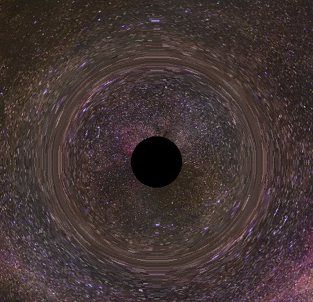
\includegraphics[width=5cm, height=5cm]{STScI-01FQHAC509H68M895P8V6R0TZP.png}
	\caption{Слева: фотография, сделанная телескопом "Хаббл"\quad\quadСправа: иллюстрация гравитационного линзирования черной дыры}
\end{figure}
\end{frame}
\begin{frame}
\begin{figure}[H]
	\centering
	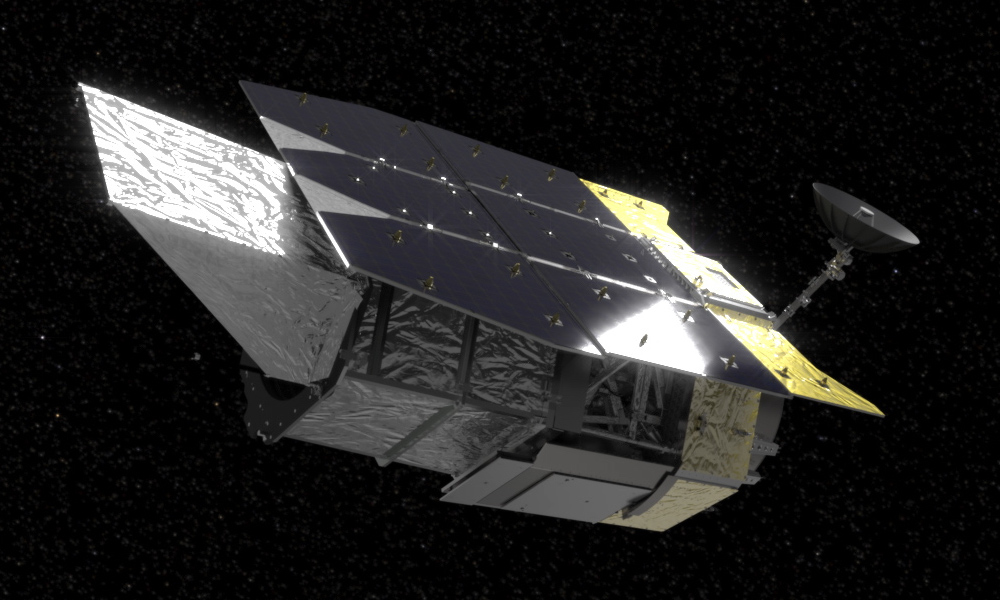
\includegraphics[width=10cm, height=7cm]{Wfirst_beauty1_prores_1920x1080mov_.00_00_17_16.still003_crop.jpg}
	\caption{Nancy Grace Roman Space Telescope}
\end{figure}
\end{frame}
\begin{frame}{Аккреционный диск и излучение}
\begin{figure}[H]
	\centering
	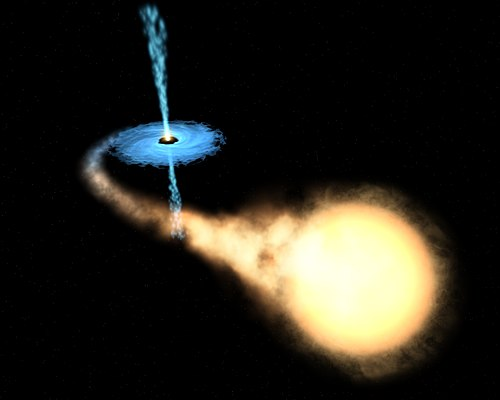
\includegraphics[width=10cm, height=7cm]{500px-accretion_disk-1.jpg}
	\caption{Аккреционный диск}
\end{figure}
\end{frame}
\begin{frame}{Аккреционный диск и излучение}
	\begin{figure}[H]
		\centering
		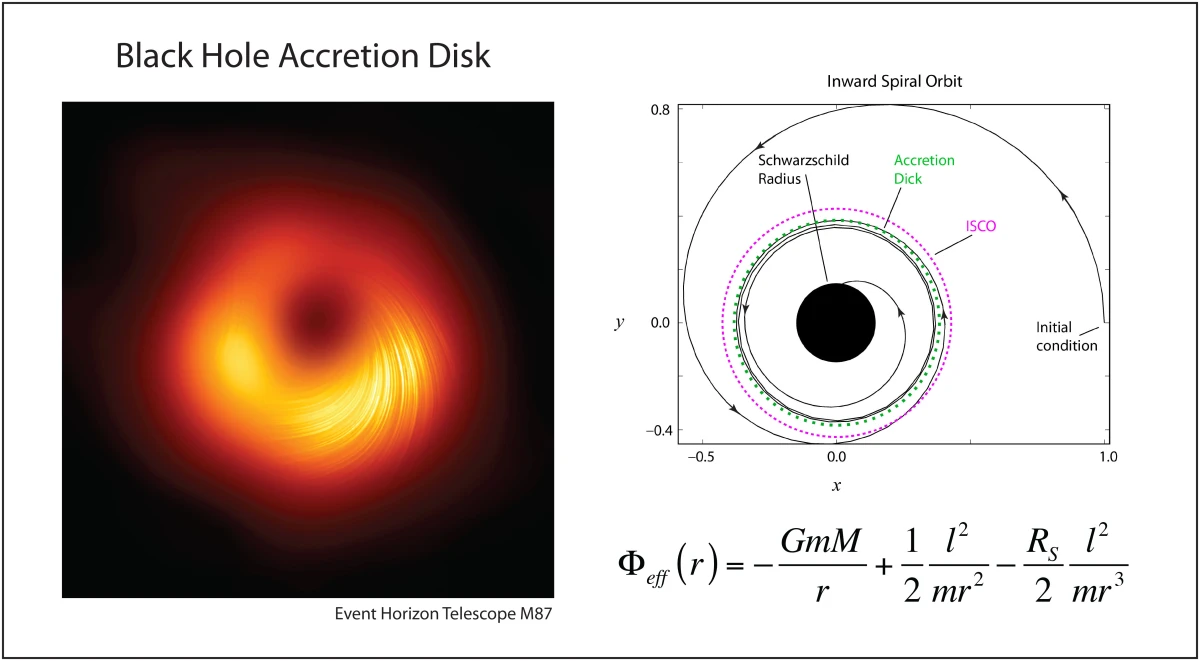
\includegraphics[width=11cm, height=6cm]{accretiondisk-2.jpg}
		\caption{Эффективный потенциал вблизи черной дыры}
	\end{figure}
\end{frame}
\begin{frame}{Джет черной дыры}
	\begin{figure}[H]
		\centering
		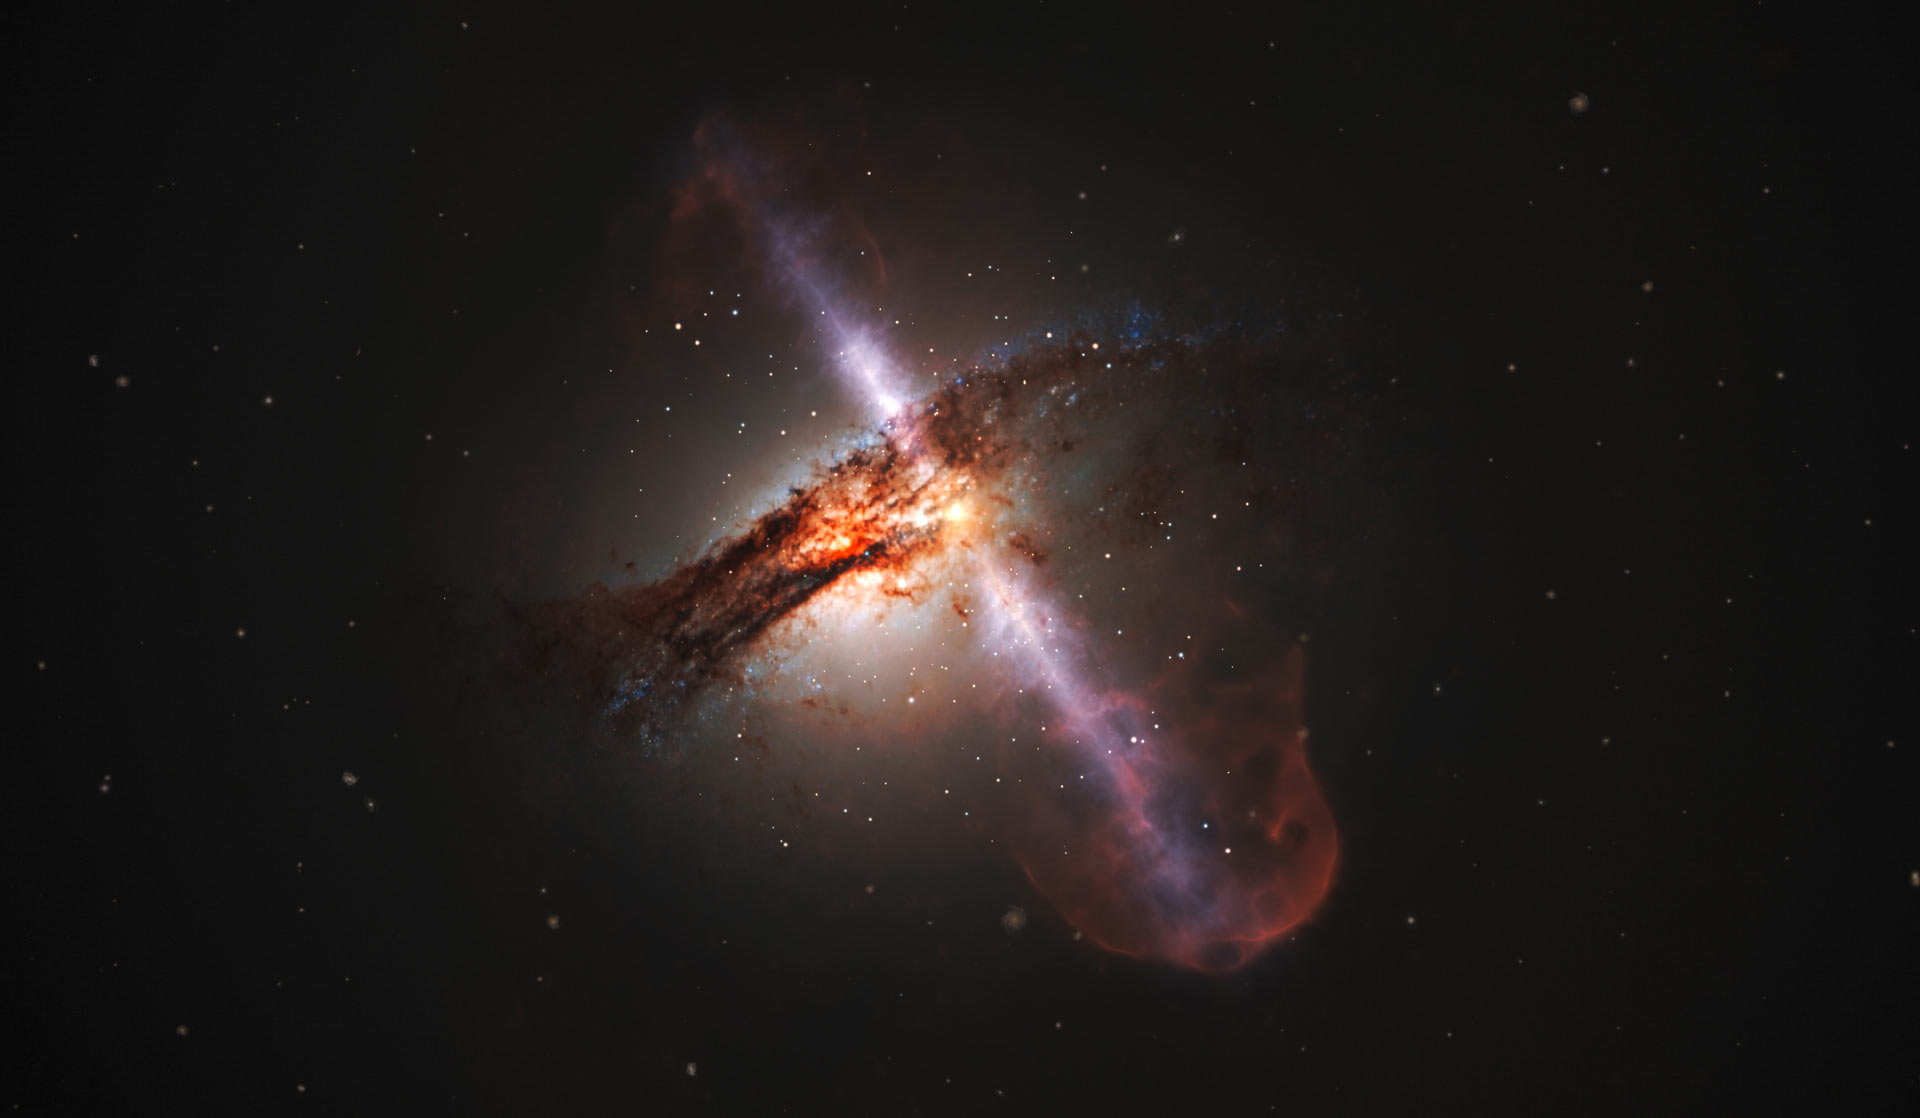
\includegraphics[width=11cm, height=7cm]{image_8308_1e-TXS-2116-077.jpg}
		\caption{Иллюстрация джета}
	\end{figure}
\end{frame}
\begin{frame}{}
	\begin{figure}[H]
		\centering
		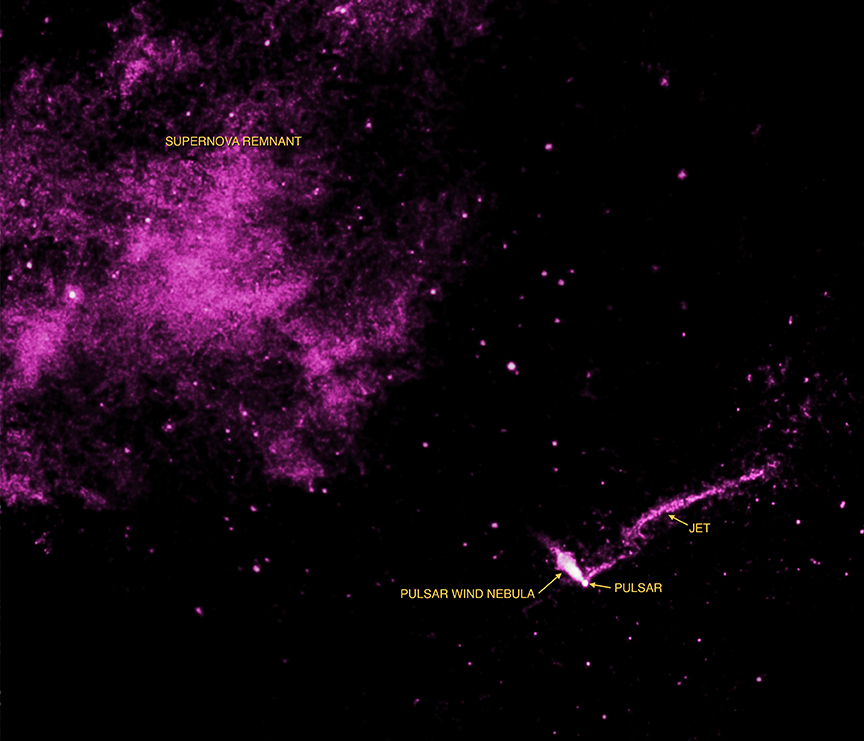
\includegraphics[width=11cm, height=7cm]{Lighthouse_nebula.jpg}
		\caption{Пульсар IGR J11014-6103}
	\end{figure}
\end{frame}
\begin{frame}{Слияние двух черных дыр}
	\begin{figure}[H]
		\centering
		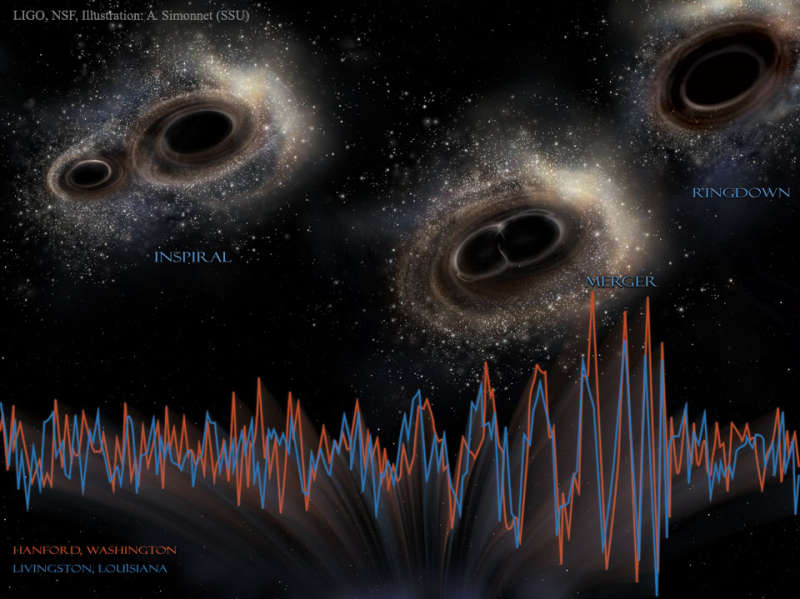
\includegraphics[width=11cm, height=7cm]{bhmerger_ligo_960.small.jpg}
		\caption{Гравитационные волны при слиянии черных дыр}
	\end{figure}
\end{frame}
\begin{frame}
\begin{center}
	Спасибо за внимание!
\end{center}
\end{frame}
\end{document}
